\section{Profile selection}
\label{design:profile_selection}

As explained in \autoref{design:overview}, the purpose of the profile selection functionality is to inform the launcher of which child profile the user wishes to launch the previously selected app with.

The ``no child selected''-state in \autoref{fig:state_diagram} shows the state of the launcher when the system is awaiting user input on which child profile to launch the previously selected app with.
%In \autoref{fig:state_diagram} the ``no child selected''-state symbolises what became profile selection.
%The \giraf[] system consists of two modes: guardian- \autoref{backlog:guardian_mode} and child mode \autoref{backlog:child_mode}.
%Herefor when in guardian mode the system do not know which child profile an app should be choosen for.
From the ``no child selected''-state, there are two transition:

\begin{enumerate}
	\item Select child
	\item Quit
\end{enumerate}

\noindent Regardless of the transition taken, the launcher will be brought  back to the ``no app selected''-state.
The difference lies on the side effects of these transitions, and therefore the behavior they produce. \\

\noindent The side effect of the \emph{select child}-transition, is the execution of the previously selected app, whereas the \emph{quit}-transaction wipes the previously select app out of memory.
%As seen in the state diagram there are two possibilities when an app have been choosen one is ``select child'' and run the app for this specific child or ``quit''.
%\subsection{Solution}

The flow chart in \autoref{fig:profileselection_design} shows the steps involved in the profile selection process.

%The profile selection feature is illustrated in \autoref{fig:profileselection_design}. 
\label{design:profile_selection}
\begin{figure}[h]
	\centering
	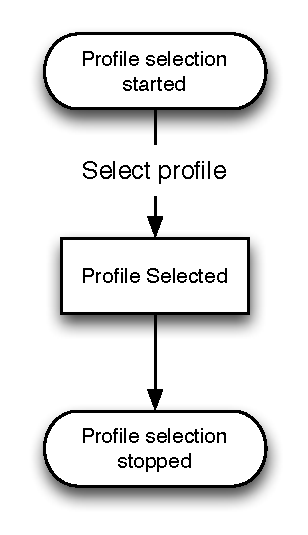
\includegraphics[width=0.6\textwidth]{gfx/profileselect_design.pdf}
	\caption{Flow chart of the profile selection process}
	\label{fig:profileselection_design}
\end{figure}

%The initial state of this feature is to choose which profile the previous selected should be launched as. This is done by clicking on the chosen profile. If the chosen profile is not visible on the screen, it can be needed to scroll through the profiles in order to find it. When the chosen profile is clicked the profile selection process is over.